\chapter{Background}
\label{chap:background}
This chapter gives a general introduction into the vocabulary of financial computing and the machine learning techniques employed.

\section{Trading Basics}
In order to understand the objective of this thesis, fundamental knowledge about the domain of financial computing is obligatory. This chapter provides a quick overview.

\subsection{Financial Instruments}
Financial instruments represent legal agreements of monetary value between parties and can be traded as assets. These assets span from  actual cash, through evidence of entity or share ownership, to contractual rights to receive or deliver another type of financial instrument.

\subsection{Markets}
Financial instruments are typically traded through one of two basic market types:
\begin{description}
\item[Over-The-Counter (OTC)] In an OTC or off-exchange market, transactions take place directly between two parties, without a mediator. Prices are negotiated directly between buyer and seller and typically not published to the public.
\item[Exchange] In exchange markets, transactions are executed by a so called broker. A broker, which can be both, an individual or a firm, executes buy and sell orders on behalf of traders for a certain fee or commission. The respective prices are determined by the current market situation, in particular by supply and demand.
\end{description}

\subsection{Exchange Markets}

Specialized exchanges concentrate on certain sub-types of financial instruments and offer a trading venue for those willing to buy and sell these instruments. Some of them are listed below:
 
\begin{description}
\item[Stock Exchange Market] A stock exchange or bourse provides companies access to investment capital in exchange to a share of ownership. Especially in times with notoriously low interest rates, investors tend to accept the greater risk of business development over a risk free, but faint investment, to grow their assets.\\
\Eg \acs{NASDAQ}, Deutsche B�rse, \dots{}
\item[Commodity exchange market] Commodity exchange markets allow for speculations with goods like oil, gold, corn, \dots{} \\
\Eg \acs{Eurex}, \dots{}
\item[Foreign exchange market] Foreign exchange (short: forex) is considered the largest financial market in the world. The forex market is responsible for determining currency exchange rates.\\
\Eg FXCM, \dots{}
\item[Digital assets exchange market] Digital asset exchange markets allow for speculations with virtual goods, like digital documents, motion picture, audible content, or digital currencies (\ie electronic money).\\
\Eg Poloniex, \dots{}
\end{description}

In the past, exchanges were physical locations. In many cases, these physical locations have been replaced by fully electronically organized markets, accessible through the internet. As a result, more traders can execute orders in a higher frequency.

\subsection{Ask and Bid}
Most exchange markets function after the so called auction market model \Cite{Klemperer99auctiontheory}, where the exchange acts as a mediator between buyers and sellers to ensure fair trading. Here buyers can \emph{bid} a price they are willing to pay for a certain number of shares and sellers can \emph{ask} a price they are aiming to make with a number of shares.
The highest of all bids is called the \emph{bid price}, the lowest of all offers is called the \emph{ask price}. Together they represent the current price at which an instrument is traded.\\

The difference between bid price and ask price is called \emph{bid-ask spread}, often abbreviated to \emph{spread}.

\subsection{Limit Order Book and Market Depth}
A limit orderbook reflects supply (asks) and demand (bids) for a particular financial instrument. It is usually maintained by the trading venue and lists the number of shares being bid or offered, organized by price levels in two opposing books. Incoming orders are constantly appended to this highly dynamic list, while a matching engine cautiously resolves any inconsistencies (\ie overlaps) between asks and bids by mediating between the involved parties.\\

It is usually not before the matching engine has arranged an actual trade, that a trading venue claims a certain percentage of the turnover as a service fee. To encourage active market participation, the pure submission, revision and cancelation of orders is typically free of charge.\\

\begin{table}
\centering
	\scalebox{0.6}{
\begin{tabular}{lrlrrr}
\toprule
{} &  Amount &    Type &  Volume &  VolumeAcc &  norm\_Price \\
\midrule
31.00 &   \color{mymauve}200.0 &     ask &  6200.0 &     8425.0 &    1.074533 \\
30.00 &    \color{mygreen}50.0 &     ask &  1500.0 &     2225.0 &    1.039871 \\
29.00 &    \color{red}25.0 &     ask &   725.0 &      725.0 &    1.005208 \\
28.85 &     NaN &  center &     NaN &        NaN &         NaN \\
28.70 &   200.0 &     bid &  5740.0 &     5740.0 &    0.994810 \\
28.50 &   100.0 &     bid &  2850.0 &     8590.0 &    0.987877 \\
28.00 &   300.0 &     bid &  8400.0 &    16990.0 &    0.970546 \\
\bottomrule
\end{tabular}}
\caption[Exemplary snapshot of a limit orderbook]{Exemplary snapshot of a limit orderbook for stocks of AIWC\protect\footnotemark}
\label{table:orderbook:example}
\end{table}
\footnotetext{Acme Internet Widget Company}

\Cref{table:orderbook:example} shows a limit orderbook snapshot up to a market depth of 3, as seen by market participants. Here Alice offers {\color{red}25} shares per 29\$, Bob and Cedar offer {\color{mygreen}20 and 30} shares respectively per 30\$ and David offers {\color{mymauve}200} shares per 31\$.\\


\label{sec:marketdata:levels}
Based on their trading needs, traders can typically choose between multiple levels of real-time market data.
\begin{description}
\item[Level 1 Market Data] Basic informations only:\\
Bid price + size, Ask price + size, Last price + size
\item[Level 2 Market Data] Additional access to the orderbook.\\
Usually data providers display the orderbook only up to a certain market depth $m$, \ie the lowest $m$ asks and the highest $m$ bids.
\item[Level 3 Market Data] Full data access.\\
Typically only accessible for the market maker.

\end{description}

\subsection{Slippage}
Slippage is defined as the difference between expected and achieved price at which a trade is executed. Slippage may occur due to delayed trade execution. Especially during periods of high volatility, markets might change faster than the order takes to be executed. Slippage is also linked to the order size, as larger orders tend to \emph{eat} into the opposing book and are fulfilled at successively worse price levels. Slippage can be both positive or negative, depending on the current market movements and must be taken into account by serious investors.


\subsection{Order Types}
\label{chap:ordertypes}
Investors can execute orders of different types, of which the most common ones are described below:

\begin{description}
\item[Market Orders] are the most simple form of orders. Here, the investor only specifies the number of shares he want's to buy/sell and the full order is executed immediately, at any price. Especially for large-scale traders or traders with level 1 data access only, these simple market orders are rather hazardous, since the achieved price can significantly differ from the expected price due to sparse supply and demand.

\item[Limit Orders] additionally feature a worst price, \ie the highest price a buyer is willing to pay per share or respectively the lowest price a seller is willing to make per share. Limit orders are immediately placed into the orderbook and (partially) executed, once the matching engine finds a corresponding trade in the opposing book.\\
Limit orders reduce the risk of slippage, but do not guarantee execution.

\item[Hidden Orders] are placed into the market makers internal orderbook, but not displayed to other market participants with level 2 market data access. They represent a simple solution to large-scale investors seeking anonymity in the market, aiming to obfuscate their trading intention from other market participants.

\end{description}

\subsection{Trading strategies}
\label{chap:tradingstrategies}
An order placement typically originates from a carefully considered \emph{trading strategy}. An \emph{active} trading strategy buys and sells instruments frequently based on short-term price movements, whereas a \emph{passive} trading strategy such as \emph{Buy-And-Hold} believes in long-term price movements eventually outweighting any short-term fluctuations.\\

As the execution of trades typically implies trading costs and slippage, these have to be taken into account. Particularly active traders with a high order quantity and large-scale investors with high order volumes are concerned with this burden. The order type chosen has a major impact on speed of execution and slippage generated.\\

While \emph{limit orders} reduce the risk of slippage, they do not guarantee full order execution. This leads to the important problem of \emph{optimized trade execution}, which frequently occurs in the domain of financial computing. In its simplest form, the problem is defined by a particular financial instrument (here: Bitcoins), which must be bought or sold within a fixed time horizon, for the best achievable share price.\\

In \cite{Nevmyvaka2005SubmitAndLeave} Nevmyvaka \etal introduce a \ac{SL}, which cleverly combines market and limit orders: After an initial limit order submission, the order is left on the market for a predefined time horizon, after which it's unexecuted part is transformed into a market order and thus executed completely. They later extended their strategy to a \ac{SR} \cite{Nevmyvaka:2006}, where the order limit may be revised at discrete time steps, depending on trade progress and market changes.

 



\section{Bitcoin}
\label{chap:bitcoins}
Bitcoin is a digital cryptocurrency, released in 2009 as open-source software under the name Satoshi Nakamoto \Cite{Davis:Bitcoin_inventor}. Motivated in part by anger over the foregone financial crisis, the underlying peer-to-peer system\Cite{Nakamoto_bitcoin:a}, provides a decentralized payment system. To this point, electronic transactions always required involving a third party to validate transactions, an inevitable necessity to forestall double-spending bitcoin tokens. Double-spending is a problem unique to digital currencies, as digital informations, in contrast to physical currencies, may be replicated arbitrarily. Rather than entrusting a central authority or central server with this validation task, a distributed public transaction log, known as the \emph{block chain}\Cite{Economist:Blockchain} is maintained among all participants.\\

The block chain is a continuously growing list of confirmed and timestamped transaction records, called \emph{blocks}. Every block includes a complex proof-of-work and a cryptographic hash of the previous block, making it extremely resistant against retrospective modifications. To motivate others to validate transactions, newly created bitcoins are rewarded to the first miner (or mining party), successfully serving the computationally demanding proof-of-work.\\

Through a manifold of legal and black markets, bitcoins may be exchanged for other currencies, products and services. In contrast to traditional exchanges, no regular trading hours exist. Transactions can be executed at all times, mostly unregulated and pseudonymous\footnote{Owners of bitcoin tokens are not explicitly identified, but bitcoin exchanges may collect personal data on their customers if required by law.}\Cite{WashingtonPost:Bitcoinfacts}. As a consequence, Bitcoin are particularly sensitive to extraordinary events or news, frequently causing immediate (panic) reactions. This effect is possibly leveraged by relatively low entry barriers, attracting amateur and professional traders likewise.

\subsection{Volatility}
\label{chap:bitcoin:volatility}
Bitcoin is a highly volatile currency, capable of massive price changes towards both directions within short periods of time. A high volatility provides profitable opportunities, but comes at the price of higher risk. Due to a very high trading volume\footnote{$\sim 40.000.000\$$ per 24h for currency pair BTC/USDT on Poloniex.\\Source: \url{https://coinmarketcap.com/exchanges/volume/24-hour} (accessed 12-July-2017)}, limit orderbooks are typically more condensed around the current best price than limit orderbooks of less frequently traded stocks. As a consequence, less slippage is to be expected from eating into the orderbook, while more slippages originates from general price fluctuations.\\

\Cref{fig:bitcoinvolatility} compares volatilities of currency pairs USDT/BTC (blue line) and USD/Pound (red line).

\begin{figure}[ht]
	\centering
	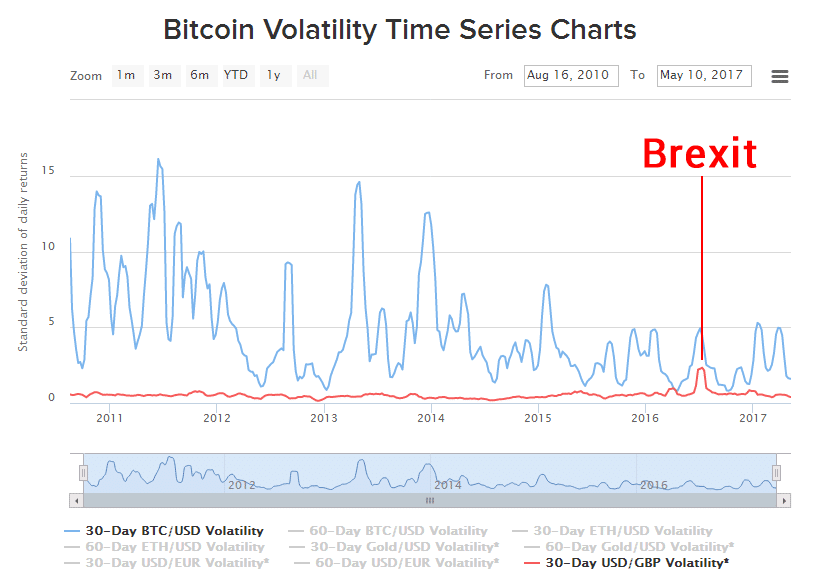
\includegraphics[width=0.6\textwidth]{content/images/BitcoinVolatility}
	\caption{BTC/USDT and USDT/Pound volatility compared..}
	\scriptsize Source: \url{https://99bitcoins.com/bitcoin-volatility-explained}
	\label{fig:bitcoinvolatility}
\end{figure}



\section{Supervised Learning}
Supervised learning is a subdomain of machine learning, where a function is learned from labeled training data $\{ (x_1, y_1), ..., (x_N, y_N) \} $. Each training sample maps a feature vectors $x_i \in X$ to a desired target value or label $y_i \in Y$. Target values may either be categorial, making the learning task a \emph{classification} problem, or continuous, making the learning task a \emph{regression} problem.

A supervised learning algorithms seeks to find a general function $g_w()$ (or it's parameters $w$), such that $g_w(x_i) \approx y_i | i \leq N$. The learned function should ideally avoid overfitting by finding a generalization to previously unseen data.


Markow Decision Process

Value Function and Bellmann Equation

Value Iteration

Q-Learning

\subsection{Logistic Regression}
bla

\subsection{Random Forest}
bla



\section{Reinforcement Learning}
Reinforcement learning is a subdomain of machine learning, where strategies are learned by an \emph{agent} interacting with its environment. Rather than learning from labeled training data, the agent applies a \emph{trial and error} pattern and exploits external rewards to find actions, maximizing his expected future reward.

\subsection{Markov Decision Process}
bla

\subsection{Value Function and Bellmann Equation}
bla

\subsection{Dynamic backward programming}
Value Iteration\\
Q-Learning

\subsection{Batch Reinforcement Learning}
bla

\subsection{Tree-Based Batch Mode Reinforcement Learning}
Randomized decision trees can be used to approximate the Q-function, as proposed by Damien Ernst \Cite{Ernst:2005:TreeBasedBatchModeRL}. The batch reinforcement learning algorithm is shown in \Cref{alg:fittedQiteration}.\\

\begin{algorithm}[H] 
 \caption{Fitted Q Iteration}
     \SetAlgoLined
          \footnotesize
     
     \KwIn{data, V, H, T, I, L}

     $\hat{Q} \leftarrow 0$\;
     \Repeat{stopping condition reached}{
      generate pattern set $P = \{(i^t, o^t) | t=1,.., n\}$ where\;
      \Indp    $i^t = (x^t, a^t),$ \hspace{0.7cm}  $o^t = r_t + \gamma * max \hat{Q}^t(s_t, u)$\;
      \Indm $\hat{Q}^{t+1} \leftarrow ^{fit} P$
     }
\label{alg:fittedQiteration}
\end{algorithm}\bigskip




\cleardoublepage{}






